\documentclass[12pt,a4paper]{article}
\usepackage{algorithm, algpseudocode, amsmath, amssymb, amsthm, bm, csquotes, emf, empheq, geometry, graphicx, hyperref, listings, mhchem, multirow, siunitx, slashbox, subcaption, upgreek}
\usepackage[italicdiff]{physics}
\usepackage[section]{placeins}
\usepackage[justification=centering]{caption}
\usepackage[column=O]{cellspace}
\usepackage[extrafootnotefeatures]{xepersian}
\hypersetup{colorlinks=true, urlcolor=cyan}

\title{تمرین سری چهارده دینامیک غیرخطی و آشوب}
\author{صالح شاملو احمدی}
\date{۲۶ خرداد ۱۴۰۲}

\settextfont{Yas}
\linespread{1.2}

\setlength\cellspacetoplimit{4pt}
\setlength\cellspacebottomlimit{3pt}
\newcommand{\multlinecell}[1]{\begin{tabular}[c]{@{}c@{}}#1\end{tabular}}

\newcommand{\qfrac}[2]{\left(\frac{#1}{#2}\right)}
\newcommand{\fsqrt}[2]{\sqrt{\frac{#1}{#2}}}
\newcommand{\ddfrac}[2]{{\displaystyle\frac{\displaystyle #1}{\displaystyle #2}}}
\newcommand{\pdvc}[3]{\qfrac{\partial #1}{\partial #2}_{#3}}
\newcommand{\dbar}{{d\mkern-7mu\mathchar'26\mkern-2mu}}
\newcommand*{\defeq}{\mathrel{\vcenter{\baselineskip0.5ex \lineskiplimit0pt
			\hbox{\scriptsize.}\hbox{\scriptsize.}}}
	=}
\DeclareMathOperator{\sign}{sgn}

\newtheorem{theorem}{قضیه}
\newtheorem{lemma}{لم}
\renewcommand\qedsymbol{$\blacksquare$}

\begin{document}
	\twocolumnfootnotes
	\maketitle
	\section{اسفنج و ابراسفنج منژر (مسئله \lr{11.3.9})}
	برای اسفنج منژر (\lr{Menger sponge}) به ازای هر شش وجه و مرکز، یک زیرمکعب کاهش می یابد. پس
	$m = 27 - 6 - 1 = 20$.
	از طرفی هر زیرمکعب سه برابر از مکعب اصلی کوچک‌تر است. پس
	\begin{equation}
		d = \frac{\ln m}{\ln r} = \frac{\ln 20}{\ln 3} \approx 2.73.
	\end{equation}
	چون حجم اسفنج منژر به صفر میل می‌کند اما سطح آن به بی‌نهایت میل می‌کند، بُعد آن باید بین $2$ و $3$ باشد
	که نشان می‌دهد عددی که برای بُعد بدست آوردیم منطقی است.
	
	برای ابراسفنج منژر (\lr{Menger hypersponge}) در $N$ بُعد، همچنان $r=3 $ و برای پیدا کردن $m$ باید الگویی
	برای تعداد زیر-ابرمکعب‌هایی که از $3^N$ زیر-ابرمکعب باقی می‌مانند پیدا کنیم. برای این منظور، هندسه مسئله را
	به مختصات تبدیل می‌کنیم تا به نوعی بتوانیم آن را کمّی کنیم. برای فرش سرپینسکی، یک عدد به ردیف و یک عدد به ستون
	نسبت می‌دهیم، طوری که جفت عدد $(x, y)$ مکان هر مربع را توصیف کند. در این صورت مربع $(2, 2)$ حذف می‌شود. اگر همین
	کار را برای اسفنج منژر با سه عدد $(x, y, z)$ تکرار کنیم، مکعب‌هایی حذف می‌شوند که حداقل دو عدد $2$ در مختصات خود
	داشته باشند. این معادل این است که هر مکعبی روی صفحه‌ای دو بُعدی در وسط قرار بگیرد، حذف می‌شود. این روش ساختن
	هر نوع ابراسفنج منژر است؛ در $N$ بُعد، اگر مختصات با حداقل دو عدد $2$ حذف شوند، مختصات باقی مانده مربوط به یک
	عدد $2$ و هیچ عدد $2$ است. برای اولی باید یک مختصه را انتخاب کنیم و برابر $2$ قرار دهیم و بقیه مختصات را برابر
	عدد $1$ یا $3$ قرار دهیم. برای دومی باید تمام مختصات را برابر عدد $1$ یا $3$ قرار دهیم. در این صورت، با استفاده
	از ترکیبیات،
	\begin{equation}
		m_N = \binom{N}{1}2^{N-1}2^{N-1} + 2^N = 2^{N-1}(N + 2),
	\end{equation}
	پس
	\begin{equation}
		d_N = \frac{\ln m_N}{\ln r} = \frac{\ln(2^{N-1}(N + 2))}{\ln 3} = \frac{(N-1)\ln 2 + \ln(N+2)}{\ln 3}.
	\end{equation}
	با استفاده از این رابطه، مطابق انتظار
	\begin{align}
		d_2 &= \frac{\ln(2^{2-1}(2 + 2))}{\ln 3} = \frac{\ln 8}{\ln 3}, \quad\checkmark \\
		d_3 &= \frac{\ln(2^{3-1}(3 + 2))}{\ln 3} = \frac{\ln 20}{\ln 3}, \quad\checkmark
	\end{align}
	و به عنوان مثال در $N=4 $
	\begin{equation}
		d_4 = \frac{\ln(2^{4-1}(4 + 2))}{\ln 3} = \frac{\ln 48}{\ln 3}.
	\end{equation}
	
	\section{نگاشت لُزی (\lr{Lozi})}
	\begin{equation}
		x_{n+1} = 1 + y_n - a\abs{x_n},\qquad y_{n+1} = bx_n
	\end{equation}
	\subsection{\lr{12.2.14}}
	مشابه نگاشت هنون (\lr{H\'enon}) تبدیل‌های $T$ تشکیل‌دهنده نگاشت را تعریف می‌کنیم:
	\begin{subequations}
		\begin{empheq}[left=\empheqlbrace]{align}
			T':& x' = x,\quad y' = 1 + y - a\abs{x} \\
			T'':& x'' = bx',\quad y'' = y' \\
			T''':& x''' = y'',\quad y''' = x''
		\end{empheq}
	\end{subequations}
	\begin{figure}[h!]
		\centering
		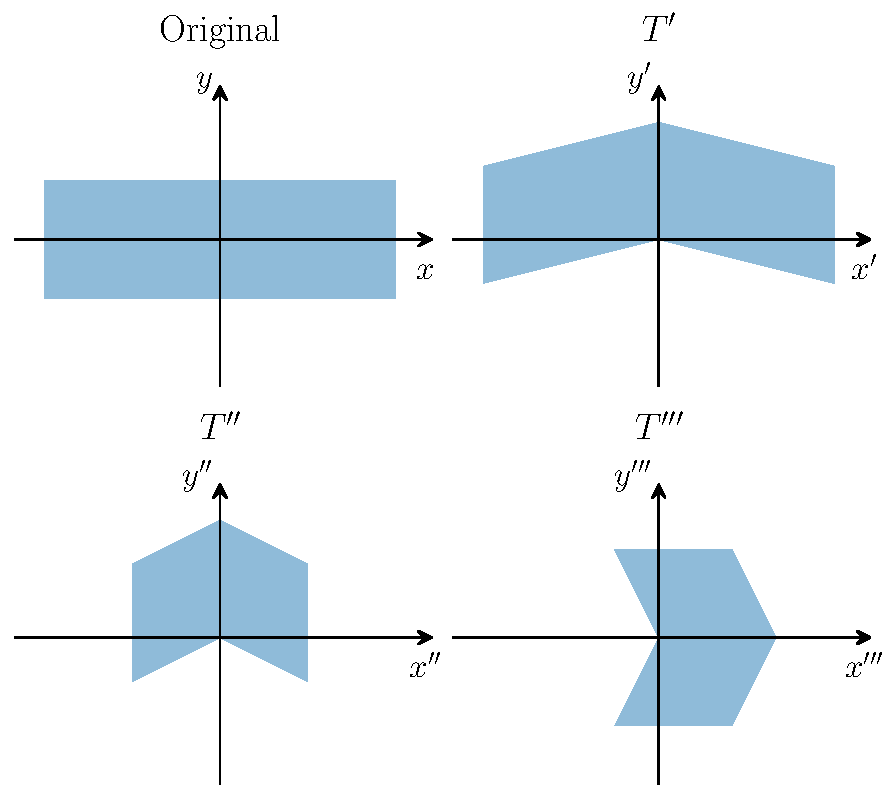
\includegraphics[width=\linewidth]{fig/12.2.14}
		\caption{مراحل اعمال نگاشت لُزی روی یک مستطیل سه در یک برای $a=0.25$ و $b=0.5$}
	\end{figure}
	\FloatBarrier
	\subsection{\lr{12.2.15}}
	ژاکوبی نگاشت لُزی برابر است با
	\begin{equation}
		J = \mqty(-a\sign(x) & 1 \\ b & 0),
	\end{equation}
	پس دترمینان $J$ که نسبت مساحت بعد به قبل اعمال نگاشت است برابر است با
	\begin{equation}
		\det(J) = -b.
	\end{equation}
	نگاشت در حالتی که
	$\abs{\det(J)} < 1$
	مساحت‌ها را کوچک می‌کند. این یعنی
	\begin{equation}
		-1 < b < 1
	\end{equation}
	\subsection{\lr{12.2.16}}
	در نقاط ثابت
	$(x_{n+1}, y_{n+1}) = (x_n, y_n) = (x^*, y^*)$.
	پس
	\begin{empheq}[left=\empheqlbrace]{align}
		x^* &= 1 + y^* - a\abs{x^*}, \\
		y^* &= bx^*,
	\end{empheq}
	\begin{subequations}
		\begin{empheq}[left={\implies\empheqlbrace}]{align}
			x^* &> 0:\quad x^* = 1 + bx^* - ax^* \implies x^* = \frac{1}{1 + a - b}, \\
			x^* &< 0:\quad x^* = 1 + bx^* + ax^* \implies x^* = \frac{1}{1 - a - b}.
		\end{empheq}
	\end{subequations}
	در آخر با رعایت خودسازگاری،
	\begin{subequations}
		\begin{empheq}[left={(x^*, y^*)=\empheqlbrace}]{align}
			\qty(\frac{1}{1 + a - b}, \frac{b}{1 + a - b}),\quad a &> b - 1,\\
			\qty(\frac{1}{1 - a - b}, \frac{b}{1 - a - b}),\quad a &> 1 - b.
		\end{empheq}
	\end{subequations}
	با استفاده از ویژه‌مقادیر ماتریس ژاکوبی برای خطی‌سازی، برای هر دو نقطه
	\begin{equation}
		\lambda_{\pm} = \frac{-a\sign(x)\pm\sqrt{a^2 + 4b}}{2}
	\end{equation}
	حال نامعادله مربوط به پایداری $\abs{\lambda_{\pm}}<1 $ را حل می‌کنیم.
	\begin{equation}
		\abs{a\sign(x)\pm\sqrt{a^2 + 4b}} < 2
	\end{equation}
	با حالت‌بندی و حل این معادله (محاسبات آن تکرار زیاد دارد و نیازی نمی‌بینم در اینجا آن را کامل بنویسم)،
	\begin{empheq}[left=\empheqlbrace]{align}
		b - 1 < a& < 1 - b, \\
		-1 < b& < 1.
	\end{empheq}
	این محدوده در صفحه $a-b$ یک مثلث با رأس‌های
	$(-1, 2)$، $(-1, -2)$
	و
	$(1, 0)$
	است. داخل این مثلث هر دو نقطه پایدار و خارج آن هر دو نقطه ناپایدار هستند.
	\subsection{\lr{12.2.17}}
	در چرخه دوتایی
	$(x_{n+2}, y_{n+2}) = (x_n, y_n) = (x, y)$،
	پس
	\begin{empheq}[left=\empheqlbrace]{align}
		x &= 1 + bx - a\abs{1 + y - a\abs{x}}, \\
		y &= b\qty(1 + y - a\abs{x}),
	\end{empheq}
	با حل این معادلات
	\begin{subequations}
		\begin{empheq}[left={(x, y)=\empheqlbrace}]{align}
			\qty(\frac{1 - a - b}{a^2 + (b-1)^2}, \frac{b(1 + a - b)}{a^2 + (b-1)^2}),\quad a &> 1 - b,\\
			\qty(\frac{1 + a - b}{a^2 + (b-1)^2}, \frac{b(1 - a - b)}{a^2 + (b-1)^2}),\quad a &> b - 1.
		\end{empheq}
	\end{subequations}
	این بار ژاکوبی برابر است با
	\begin{equation}
		J = \mqty(b + a^2\sign\qty(x\qty(1+y-a\abs{x})) & -a\sign(x) \\ -ab\sign(x) & b)
	\end{equation}
	که در نقطه اول برابر است با
	\begin{equation}
		J_1 = \mqty(b - a^2 & -a \\ ab & b)
	\end{equation}
	و در نقطه دوم برابر است با
	\begin{equation}
		J_1 = \mqty(b - a^2 & a \\ -ab & b).
	\end{equation}
	با بدست آوردن ویژه‌مقادیر
	\begin{equation}
		\lambda_{\pm} = \frac{-a^2 + 2b \pm a\sqrt{a^2 - 4b}}{2}
	\end{equation}
	و با حل نامعادله پایداری $\abs{\lambda_{\pm}}<1 $ محدوده پایداری بدست می‌آید
	\begin{empheq}[left=\empheqlbrace]{align}
		1 - b < a& < 1 + b, \\
		0 < b& < 1,
	\end{empheq}
	که در صفحه $a-b$ مثلثی است با رأس‌های
	$(1, 0)$، $(1, 2)$
	و
	$(0, 1)$.
	\FloatBarrier
	\subsection{\lr{12.2.18}}
	\begin{figure}[h!]
		\centering
		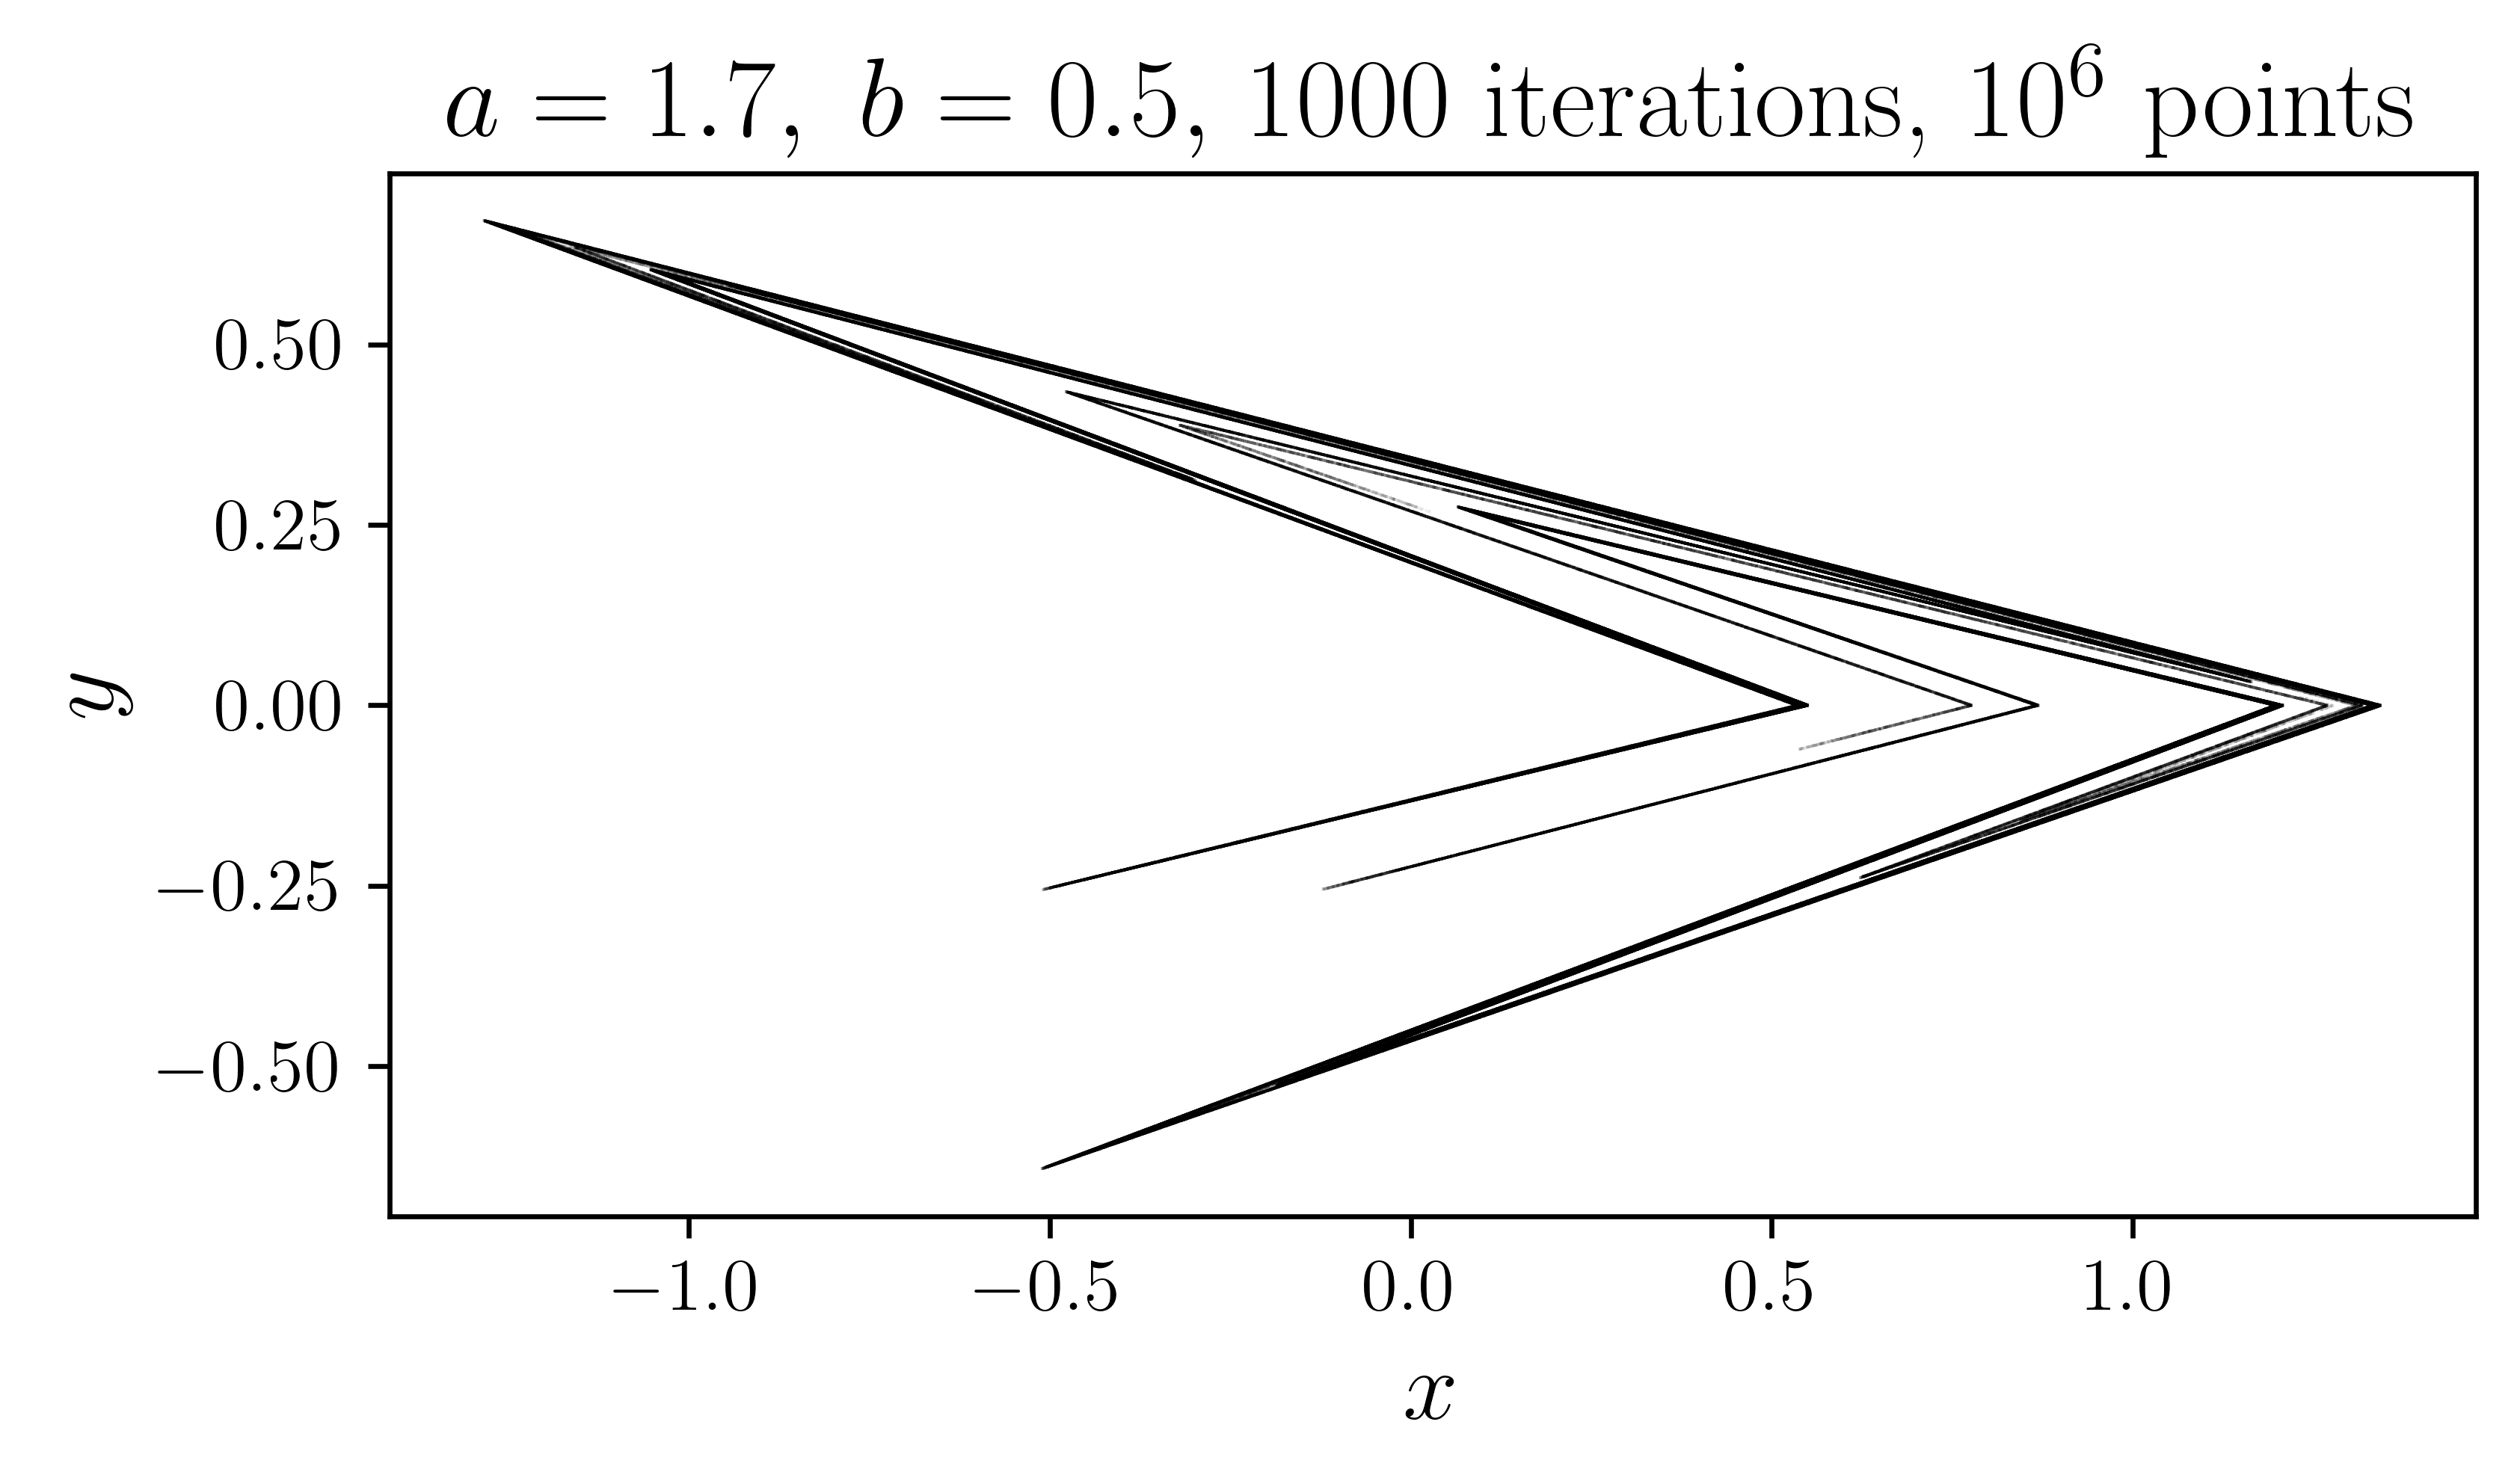
\includegraphics[width=\linewidth]{fig/12.2.18}
		\caption{ساختار فراکتالی مربوط به رباینده عجیب در شکل دیده می‌شود.}
	\end{figure}
	
	\section{سیستم روسلر}
	\subsection{\lr{12.3.1, a)}}
	برای درست کردن نمودار دوشاخگی، $x$های مثبتی که در آن‌ها $y$ تغییر علامت می‌دهد را برحسب $a$ رسم می‌کنیم.
	این نوعی مقطع از سیستم می‌دهد که تحلیل آن را ساده‌تر می‌کند.
	
	با توجه به نمودار و زومی که روی آن انجام شده، دوشاخگی \lr{Hopf} در حدود
	$a=0.3357$
	است و اولین دوشاخگی دوبرابرکننده دوره تناوب در حدود
	$a=0.37483$
	است.
	\begin{figure}[h!]
		\centering
		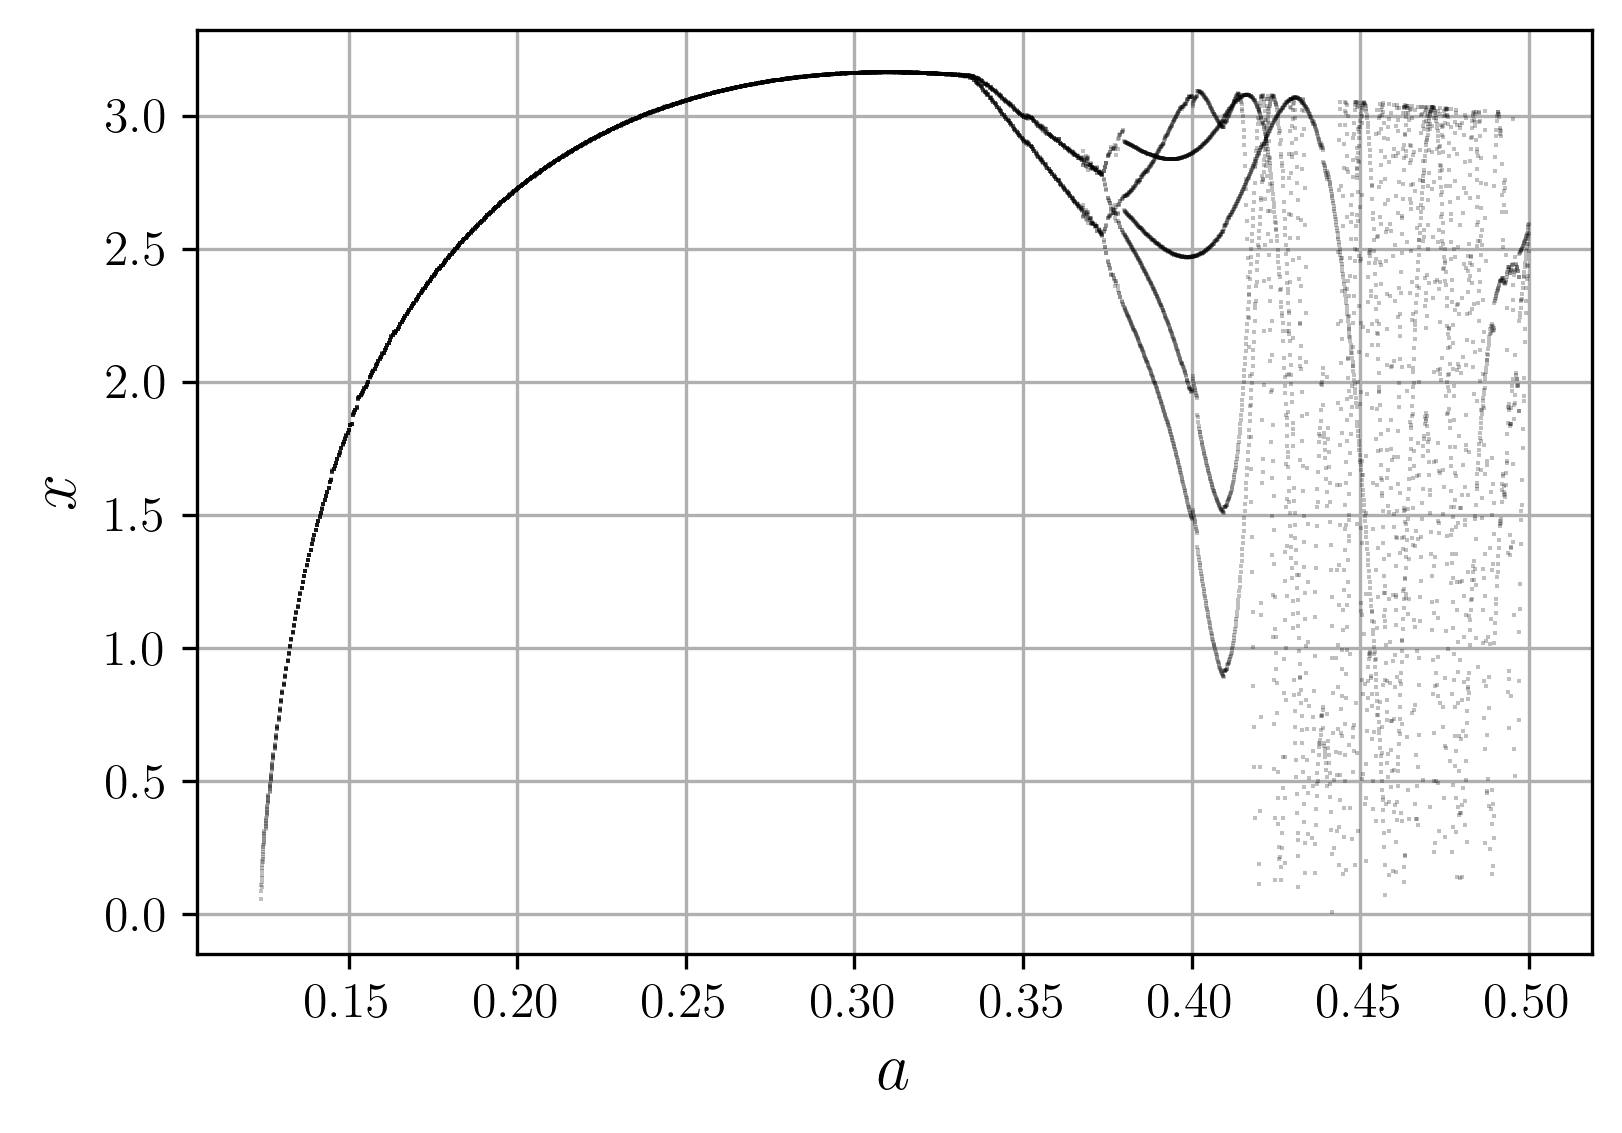
\includegraphics[width=\linewidth]{fig/12.3.1.bifurcation}
		\caption{نمودار دوشاخگی}
	\end{figure}
	\begin{figure}[h!]
		\begin{subfigure}{0.49\linewidth}
			\centering
			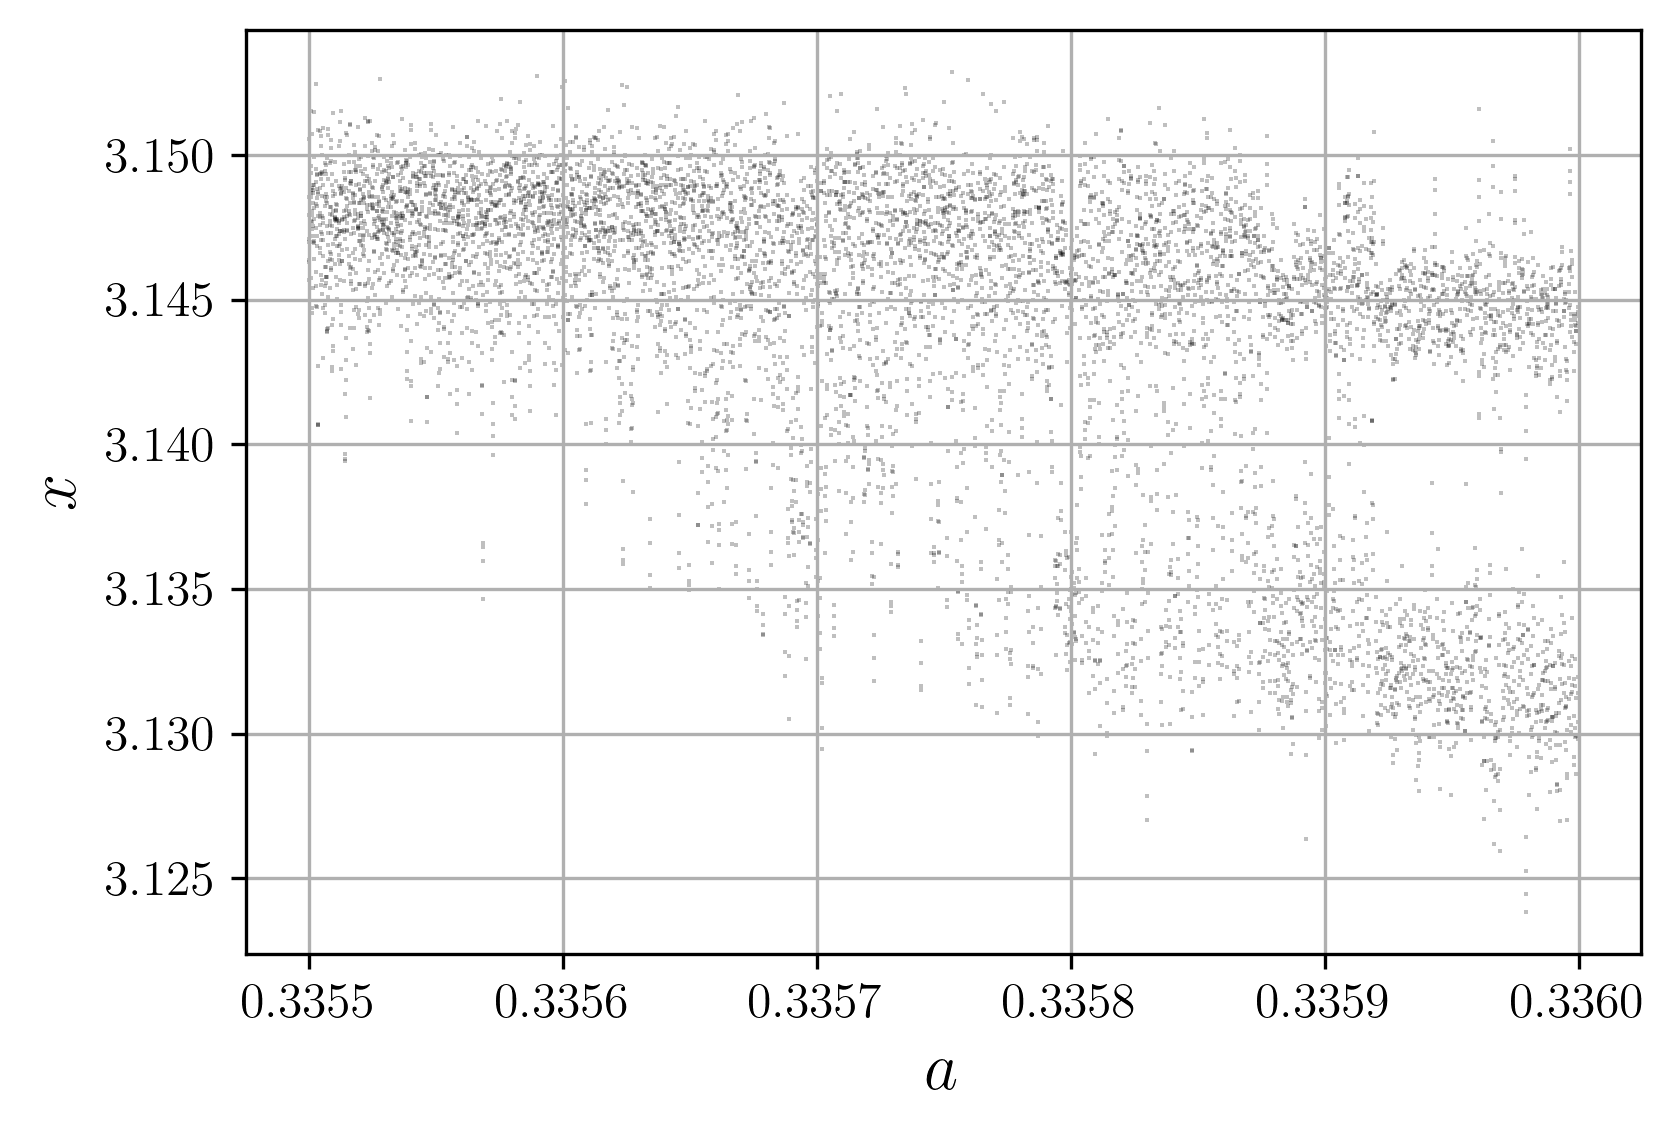
\includegraphics[width=\linewidth]{fig/12.3.1.zoom.hopf}
			\caption{زوم روی دوشاخگی \lr{Hopf}}
		\end{subfigure}
		\begin{subfigure}{0.49\linewidth}
			\centering
			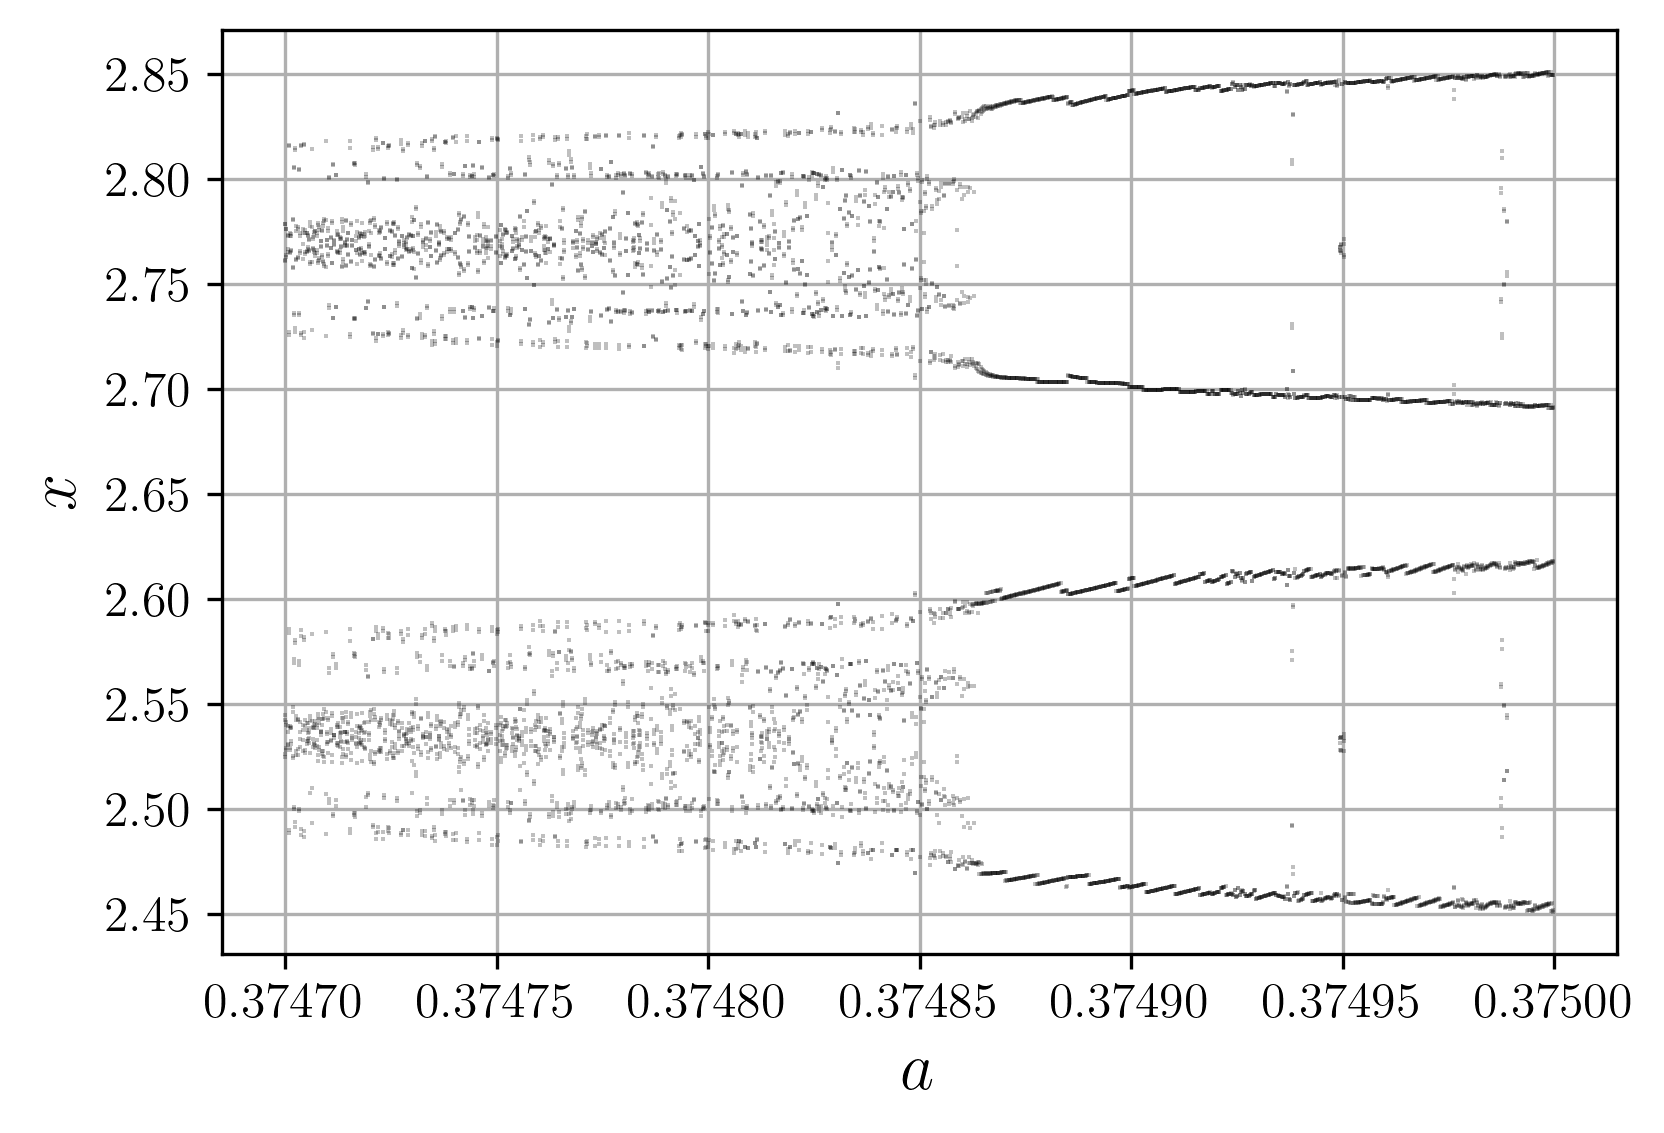
\includegraphics[width=\linewidth]{fig/12.3.1.zoom.double}
			\caption{زوم روی اولین دوشاخگی دوبرابرکننده دوره تناوب.}
		\end{subfigure}
	\end{figure}

	\FloatBarrier
	\subsection{\lr{12.3.1, b)}}
	\begin{figure}[h!]
		\centering
		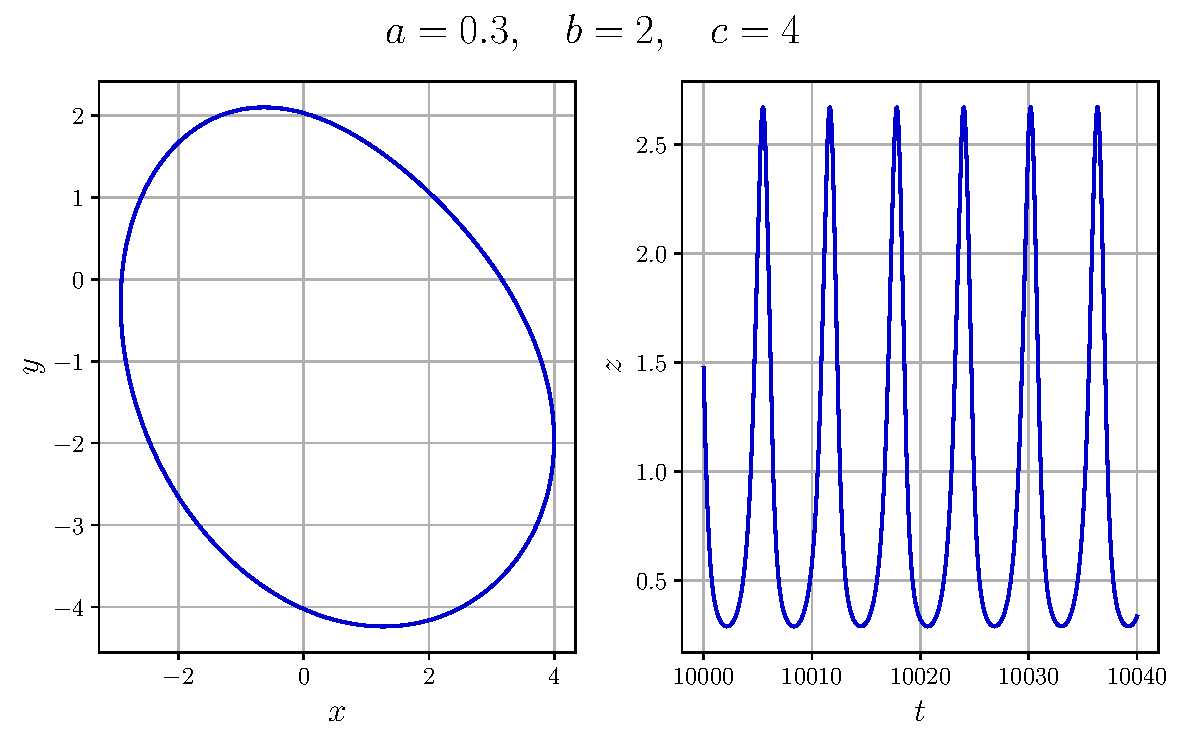
\includegraphics[width=\linewidth]{fig/12.3.1.normal}
		\caption{قبل از دوشاخگی \lr{Hopf}}
	\end{figure}
	\begin{figure}[h!]
		\centering
		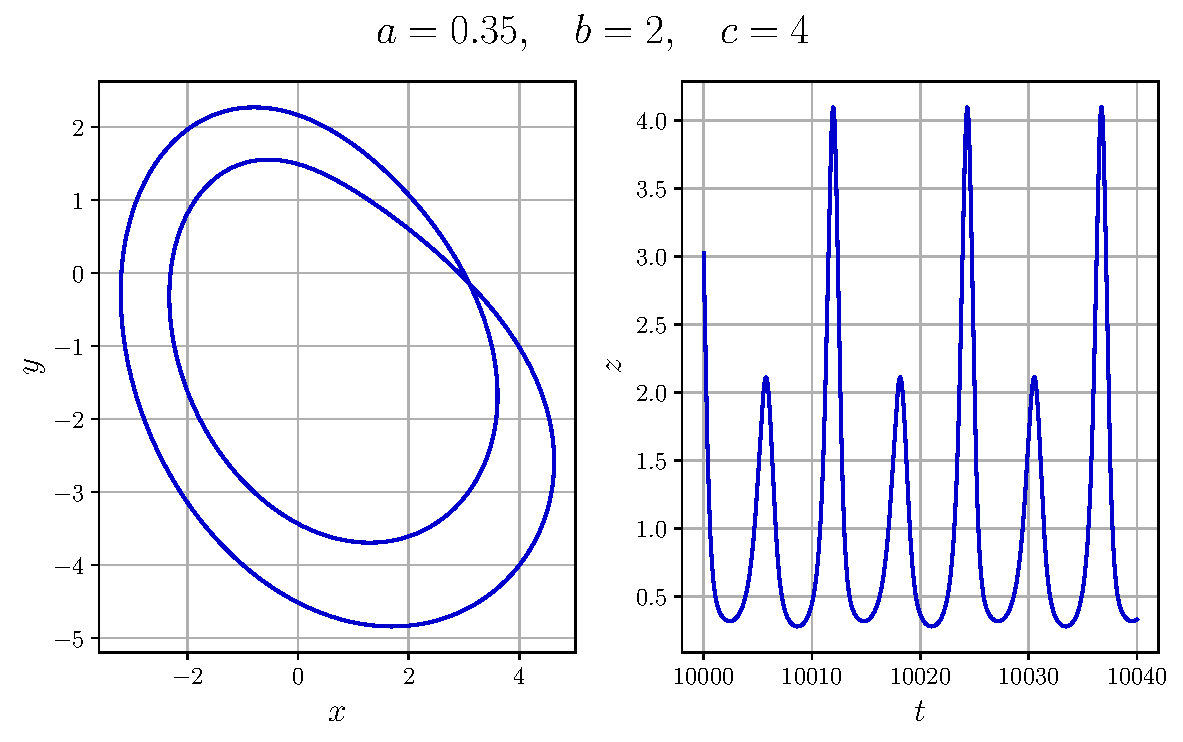
\includegraphics[width=\linewidth]{fig/12.3.1.hopf}
		\caption{بعد از دوشاخگی \lr{Hopf} و قبل از دوشاخگی دوبرابرکننده دوره تناوب.}
	\end{figure}
	\begin{figure}[h!]
		\centering
		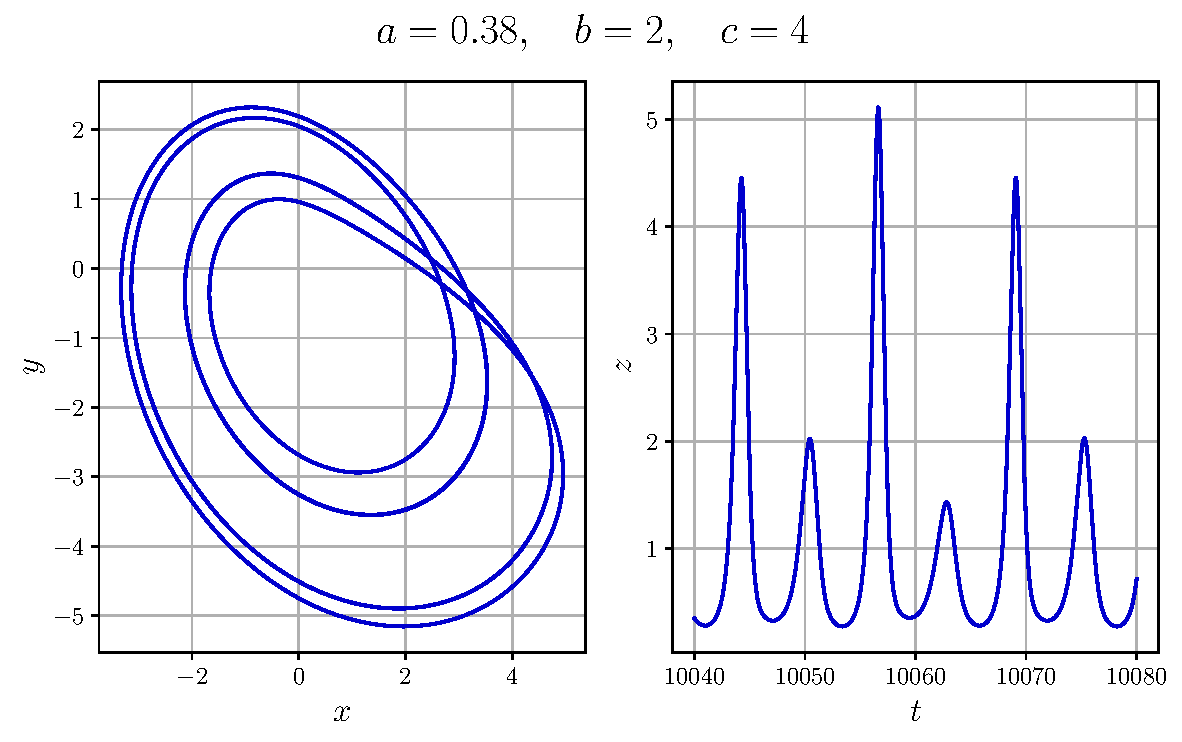
\includegraphics[width=\linewidth]{fig/12.3.1.double}
		\caption{بعد از اولین دوشاخگی دوبرابرکننده دوره تناوب.}
	\end{figure}
\end{document}